\documentclass[french,12pt]{article}
\usepackage[a4paper,margin=1in]{geometry}
\usepackage{babel}
\usepackage[T1]{fontenc}
\usepackage[utf8]{inputenc}
\usepackage{enumitem}
\usepackage{graphicx,wrapfig}
\usepackage{listings}
\usepackage{inconsolata}
\usepackage[font=scriptsize,justification=centering,margin=.5cm]{caption}

\lstset{
	basicstyle=\small\ttfamily,
	breaklines=true,
	extendedchars=true,
	tabsize=4
}

\graphicspath{ {./data/img/} }

% \setlength{\parindent}{0pt}

\newcounter{qnum}
\def\question{\par\medskip\refstepcounter{qnum}{\bfseries Question \arabic{qnum}. }}

\begin{document}

\begin{titlepage}
		\centering
		
\includegraphics[width=.25\textwidth]{logo.png}\par\vspace{1.5cm}
		{\scshape\large Master 1 - ANDROIDE \par}
		\vspace{.5cm}
		{\scshape\Large Robotique et Apprentissage\par}
		\vspace{1.5cm}
		{\LARGE\bfseries Coding and study of regression algorithms\par}
		\vspace{2cm}
		{\large\itshape Julien Canitrot, Jules Dubreuil\par}

		\vspace{.5cm}
		
		supervisé par\par
		Olivier \textsc{Sigaud}

		\vspace{1.5cm}
		
		\tableofcontents

		\vfill

		{\today\par}
\end{titlepage}


\section{Batch Linear Least squares}

\subsection{Linear least squares}

%Q1
\question Does \lstinline{your train(self, x_data, y_data)} function provide exactly the same results as the \lstinline{train_from_stats(self, x_data, y_data)} function? Call both functions 2000 times. Is one faster than the other?
\medskip

\begin{lstlisting}
[Out] 	LLS average time: 1.344e-03s
	  	LLS from scipy stats average time: 1.233e-03s
	  	results proximity (tolerance of 1e-08): 100.0%
\end{lstlisting}

\noindent Le temps d'exécution est du même ordre de grandeur pour les deux fonctions, avec un légère avantage pour notre implémentation.
Les résultats sont quasiment identiques. La très légère différence est due au fait que notre implémentation fait un arrondi de $\theta$ à $10^{-7}$.

\subsection{Ridge Regression}

%Q2
\question For a batch of 50 points, study with the \lstinline{train_regularized(self,x_data,y_data,coef)} function how the residuals degrade as you increase the value of coef. A good idea would be to make a picture with coef in the x axis and the residuals in the y axis, and then to comment on it.
\bigskip

Les deux figures ci-dessous représentent l'impact de la valeur du coefficient sur l'erreur (les résidus) de LRR, sur une moyenne de 20 batchs de 50 points.

\begin{figure}[ht]
\centering
\begin{minipage}{.45\textwidth}
	\centering
	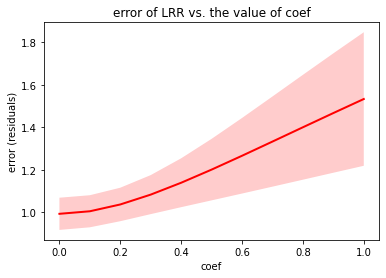
\includegraphics[width=\textwidth]{LRR_error_vs_coef1.png}
	\captionof{figure}{Evolution de l'erreur pour un coefficient allant de 0 à 1.}
	\label{fig:LRR_error_vs_coef1}
\end{minipage}
\hfill
\begin{minipage}{.45\textwidth}
	\centering
	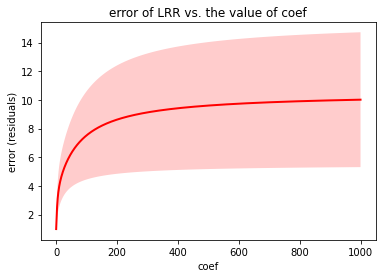
\includegraphics[width=\textwidth]{LRR_error_vs_coef1000.png}
	\captionof{figure}{Evolution de l'erreur pour un coefficient allant de 0 à 1000.}
	\label{fig:LRR_error_vs_coef1000}
\end{minipage}
\end{figure}

Par lecture graphique, on comprend que plus le coefficient s'éloigne de 0 moins le résultat est précis. Cependant l’erreur augmente de moins en moins au fur et à mesure qu'on augmente le coefficient.
En effet pour des valeurs de \lstinline{coef} de 0.1 à 1 l’erreur résiduelle augmente linéairement. Pour des valeurs de \lstinline{coef} de 1 à 1000 elle augmente beaucoup plus lentement.

\clearpage
\begin{wrapfigure}[11]{r}{.5\textwidth}
% \centering
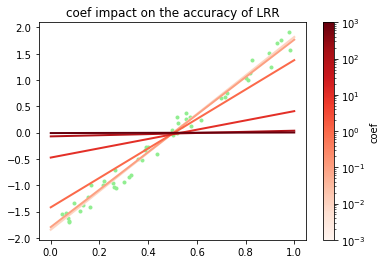
\includegraphics[width=.5\textwidth]{LRR_coef_impact.png}
% \captionof{figure}{Impact du coefficient sur la précision de LRR.}
% \label{fig:LRR_coef_impact}
\end{wrapfigure}

La figue (ci-contre) permet de bien mettre en évidence la corrélation entre l'augmentation du coef et la baisse de précision du résultat.

Lorsque le coefficient tend vers l'infini, l'allure de la courbe va tendre vers l'horizontal.
Ainsi, moins le résultat est précis, moins le fait d’augmenter le coefficient aura un impact sur l'allure de la courbe.

C’est pourquoi après un coefficient de 100, l’erreur n’augmente quasiment plus.
% Ainsi, lorsque le coefficient est de l'odre de $10^2$, le résultat sera suffisament imprécis pour que l'augmenter de nouveau n'ait pas un impact significatif sur l'allure de la courbe.
\bigskip

% \newpage
\section{Radial Basis Function Networks}

\subsection{Batch RBFNs}

%Q3
\question Call the train functions at least 1000 times, comment on the difference in computation time between the first and the second perspective.
\medskip

\begin{lstlisting}
[Out] 	First strategy average time: 8.312e-04s
		Second strategy average time: 5.261e-03s
\end{lstlisting}

La première stratégie est plus rapide que la deuxième d'un facteur 10. Cela pourrait s'expliquer par l'utilisation d'une boucle \lstinline{for} dans la deuxième stratégie qui à tendance à réduire l'efficacité des algorithmes.
\bigskip

%Q4
\question Study the evolution of the error as a function of the number of features. A good idea would be to make a picture with the number of features in the x axis and the residuals in the y axis, and then comment on it. Have a look at the model when the number of features is large (e.g. 30). What is happening?

\begin{figure}[ht]
\centering
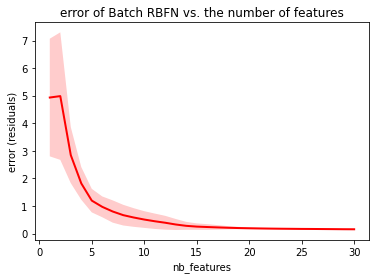
\includegraphics[width=.45\textwidth]{batch_rbfn_error_vs_n_features30.png}
\captionof{figure}{Evolution du temps de calcul de RLS pour un nombre de features allant de 1 à 30.}
\label{fig:batch_rbfn_error_vs_nfeat30}
\end{figure}

Encore une fois on peut observer que plus le nombre de features est grand, plus le modèle devient précis (Figure \ref{fig:batch_rbfn_error_vs_nfeat30}). Nous discutons du comportement du modèle aux alentours de 60 features en Annexes.

% Cela se retranscrit sur les figures ci-dessous.

\begin{figure}[ht]
\centering
\begin{minipage}{.45\textwidth}
	\centering
	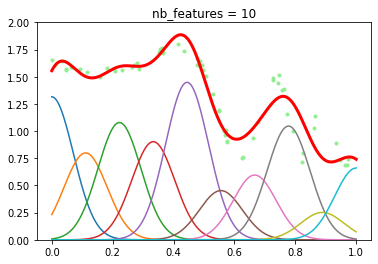
\includegraphics[width=\textwidth]{overfitting_10.png}
	\captionof{figure}{Prédiction du modèle RLS pour\\ 10 features (underfitting entre 0.6 et 1).}
	\label{fig:overfitting_10}
\end{minipage}
\hfill
\begin{minipage}{.45\textwidth}
	\centering
	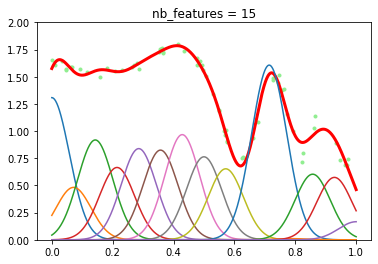
\includegraphics[width=\textwidth]{overfitting_15.png}
	\captionof{figure}{Prédiction du modèle RLS pour\\ 15 features (restes d'underfitting).}
	\label{fig:overfitting_15}
\end{minipage}
\begin{minipage}{.45\textwidth}
	\centering
	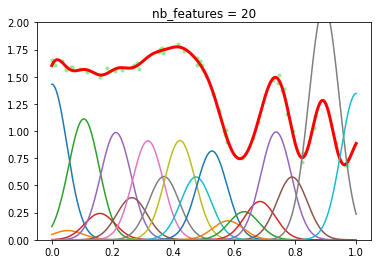
\includegraphics[width=\textwidth]{overfitting_20.png}
	\captionof{figure}{Prédiction du modèle RLS pour\\ 20 features (début d'overfitting).}
	\label{fig:overfitting_20}
\end{minipage}
\hfill
\begin{minipage}{.45\textwidth}
	\centering
	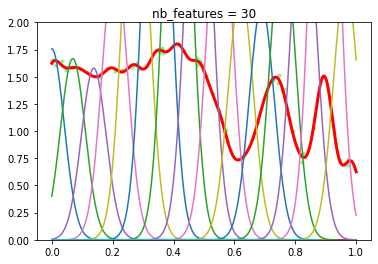
\includegraphics[width=\textwidth]{overfitting_30.png}
	\captionof{figure}{Prédiction du modèle RLS pour\\ 30 features (overfitting entre 0 et 0.6).}
	\label{fig:overfitting_30}
\end{minipage}
\end{figure}

La corrélation entre le nombre de features et la précision se retrouve sur les figures ci-dessus. Pour 10 features le modèle ne donne pas une bonne approximation de la fonction latente entre 0.6 et 1 (underfitting). Au contraire, pour 30 features le modèle fait de l'overfitting (Figure \ref{fig:overfitting_30}) : il ne prend pas en compte qu'il puisse y avoit une variance dans la position des points, il ne décrit donc plus la fonction à approximer mais fait de l'apprentissage par c\oe{ur}.

Sur cette exemple, la meilleure approximation semble se trouver entre 15 et 20 features (Figures \ref{fig:overfitting_15} et \ref{fig:overfitting_20}).

\subsection{Incremental RBFNs}

%Q5
\question By varying the number of features, the number of samples and the amount of noise in the data generator, compare both recursive variants (with and without the Sherman-Morrison formula) and gradient descent. Which is the most precise? The fastest? Using graphical displays where you are varying the above parameters is strongly encouraged.

\clearpage
\begin{figure}[ht]
\centering
\begin{minipage}{.33\textwidth}
	\centering
	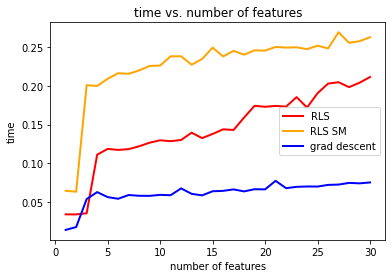
\includegraphics[width=\textwidth]{time_vs_n_features.png}
	\captionof{figure}{Evolution du temps de calcul en fonction du nombre de features.}
	\label{fig:rbfn_time_vs_nfeat}
\end{minipage}
\hfill
\begin{minipage}{.33\textwidth}
	\centering
	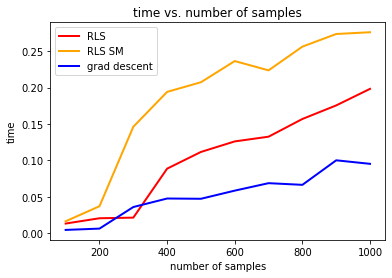
\includegraphics[width=\textwidth]{time_vs_n_samples.png}
	\captionof{figure}{Evolution du temps de calcul en fonction du nombre d'échantillons.}
	\label{fig:rbfn_time_vs_nsamp}
\end{minipage}\hfill
\begin{minipage}{.33\textwidth}
	\centering
	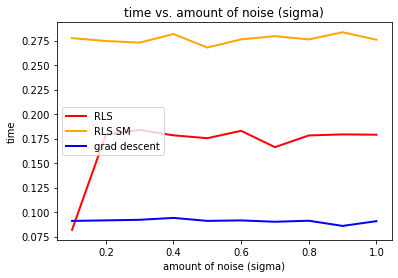
\includegraphics[width=\textwidth]{time_vs_noise.png}
	\captionof{figure}{Evolution du temps de calcul en fonction de la quantité de bruit.}
	\label{fig:rbfn_time_vs_noise}
\end{minipage}
\end{figure}

Augmenter le nombre de features fait croître le temps de calcul de chaque modèle de façon linéaire.

On remarque surtout qu'il y a une nette différence de performances entre les 3 méthodes de calcul (Figure \ref{fig:rbfn_time_vs_nfeat}, \ref{fig:rbfn_time_vs_nsamp} et \ref{fig:rbfn_time_vs_noise}). RLS Sherman Morrison est plus long que son homologue qui est lui même plus long que la méthode par descente de gradient. Cela s’explique par le fait que pour les méthodes RLS nous devons faire une inversion de matrice ce qui n’est pas le cas pour la descente de gradient.

Sur la dernière figure (Figure \ref{fig:rbfn_time_vs_noise}) on remarque que la quantité de bruit n'influe pas sur le temps de calcul ($\sigma=0$ provoquant un effet de bord).

\begin{figure}[ht]
\centering
\begin{minipage}{.45\textwidth}
	\centering
	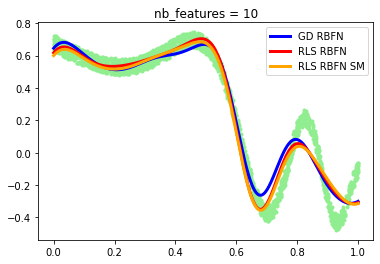
\includegraphics[width=\textwidth]{incr_rbfn_10feat.png}
	\captionof{figure}{Prédiction des modèles pour\\ 10 features.}
	\label{fig:incr_rbfn_10feat}
\end{minipage}
\hfill
\begin{minipage}{.45\textwidth}
	\centering
	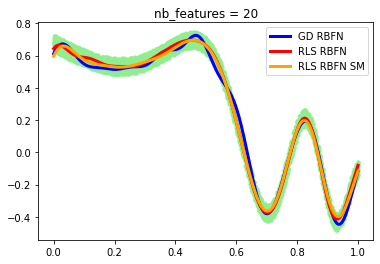
\includegraphics[width=\textwidth]{incr_rbfn_20feat.png}
	\captionof{figure}{Prédiction des modèles pour\\ 20 features.}
	\label{fig:incr_rbfn_20feat}
\end{minipage}
\begin{minipage}{.45\textwidth}
	\centering
	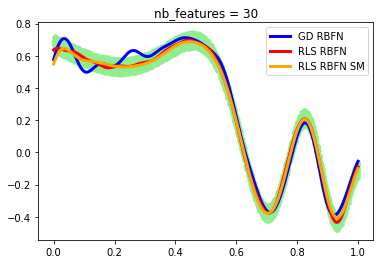
\includegraphics[width=\textwidth]{incr_rbfn_30feat.png}
	\captionof{figure}{Prédiction des modèles pour\\ 30 features.}
	\label{fig:incr_rbfn_30feat}
\end{minipage}
\hfill
\begin{minipage}{.45\textwidth}
	\centering
	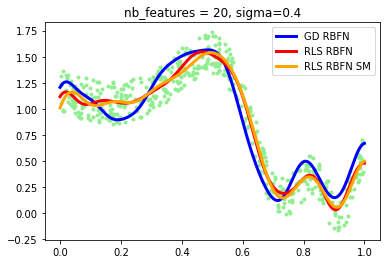
\includegraphics[width=\textwidth]{incr_rbfn_sigma.png}
	\captionof{figure}{Prédiction des modèles pour\\ 20 features et $\sigma = 0.4$.}
	\label{fig:incr_rbfn_sigma}
\end{minipage}
\end{figure}

Sur les figures \ref{fig:incr_rbfn_10feat}, \ref{fig:incr_rbfn_20feat}, \ref{fig:incr_rbfn_30feat} on observe que le nombre de features permet d'augmenter la précision. Cependant on remarque que chaque algorithme réagit différement. En effet, à partir de 20 features la méthode descente de gradient commence déjà à overfitter. Cela ne va pas en s'améliorant, et à 30 features RLS overfit aussi. La version Sherman Morisson quant à elle ne subit pas trop de variations.

Par ailleurs, avec l’aide de la Figure \ref{fig:incr_rbfn_sigma} on constate que la descente de gradient est très sensible au bruit. RLS est moins sensible, mais encore une fois c’est RLS SM qui est le plus performant dans ce domaine.

Pour conclure, la méthode Sherman Morrison est plus précise dans la majorité des situations mais souffre d'un temps de calcul supérieur aux deux autres méthodes. La méthode de descente de gradient, à l'inverse, est très rapide mais moins précise, et souffre d'overfitting. La méthode RLS simple est un compromis entre les deux.
\bigskip

%Q6
\question Using RBFNs, comment on the main differences between incremental and batch methods. What are their main advantages and disadvantages? Explain how you would choose between an incremental and a batch method, depending on the context.
\medskip

La différence majeure entre les méthodes incrémentales et Batchs est la flexibilité sur la gestion du temps de calcul.

Pour un nombre de features fixé, la méthode Batch prend un set de $N$ données d'un seul coup, ce qui rend un résultat plus précis.
Cependant, dû à l'inversion de matrice le temps de calcul est en $O(N^3)$, ce qui est beaucoup trop cher pour des gros sets de données.

Les méthodes RLS (avec ou sans variante Sherman Morrison) réalisent une inversion de matrice incrémentale, ce qui permet de réduire la complexité en $O(N^2)$. La méthode de descente de gradient, quant à elle, n'a pas besoin d'inversion de matrice. De plus, il est possible de modifier le nombre d'itérations ainsi que la taille des mini-batchs, au détriment de la précision.

Les méthodes incrémentales offrent donc une flexibilité sur la précision, tout en ayant des temps de calcul nettement plus faibles que les méthodes Batch sur des gros sets de données.

On favorisera donc les méthodes Batchs pour des petits sets de données, afin de valoriser la précision, et les méthodes incrémentales pour les gros sets afin d'éviter des temps de calcul trop longs.

\newpage
\section{Locally Weighted Regression}

%Q7
\question Study the impact of \lstinline{nb_features} on the accuracy of LWR. As usual, make a drawing where you measure the residuals as a function of the number of features.

\begin{figure}[h]
	\centering
	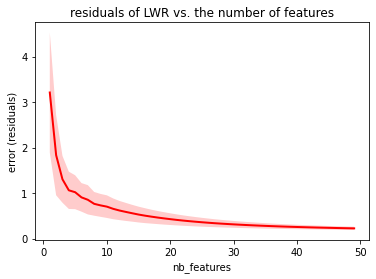
\includegraphics[width=.45\textwidth]{LWR_error_vs_n_features.png}
	\captionof{figure}{Erreur de LWR en fonction du nombre de features.}
	\label{fig:LWR_error_vs_n_features}
\end{figure}

De la même manière que pour les autres modèles, on peut conclure qu'augmenter le nombre de features de LWR permet de réduire l'erreur (Figure \ref{fig:LWR_error_vs_n_features}).

\begin{figure}[ht]
\centering
\begin{minipage}{.45\textwidth}
	\centering
	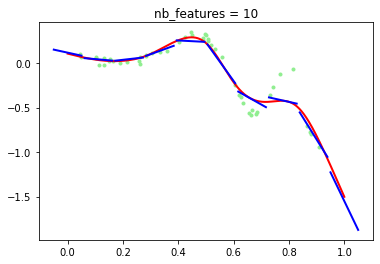
\includegraphics[width=\textwidth]{lwr_nfeat_10.png}
	\captionof{figure}{Prédiction de LWR pour\\ 10 features.}
	\label{fig:lwr_nfeat_10}
\end{minipage}
\hfill
\begin{minipage}{.45\textwidth}
	\centering
	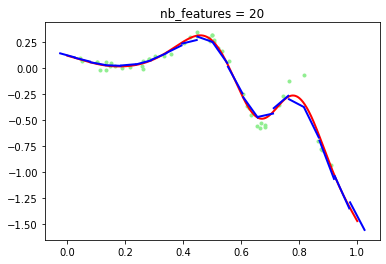
\includegraphics[width=\textwidth]{lwr_nfeat_20.png}
	\captionof{figure}{Prédiction de LWR pour\\ 20 features.}
	\label{fig:lwr_nfeat_20}
\end{minipage}
\begin{minipage}{.45\textwidth}
	\centering
	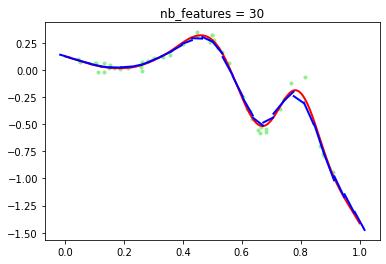
\includegraphics[width=\textwidth]{lwr_nfeat_30.png}
	\captionof{figure}{Prédiction de LWR pour\\ 30 features.}
	\label{fig:lwr_nfeat_30}
\end{minipage}
\hfill
\begin{minipage}{.45\textwidth}
	\centering
	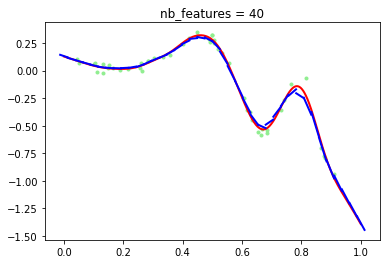
\includegraphics[width=\textwidth]{lwr_nfeat_40.png}
	\captionof{figure}{Prédiction de LWR pour\\ 40 features.}
	\label{fig:lwr_nfeat_40}
\end{minipage}
\end{figure}

Sur ces figures on remarque que 10 features semblent être trop justes pour atteindre une approximation satisfaisante. Cependant cette approximation continue d’augmenter en précision sans tomber dans l’overfitting.

Cela s’explique par le fait que nous utilisons des parties linéaires pour approximer la fonction. En effet, ces segments ayant une taille non négligeable, le modèle aura tendance à faire une moyenne des points et à ne pas subir la variance des données. Ainsi pour les expérimentations avec beaucoup de bruit cette méthode est particulièrement efficace.

\begin{figure}[ht]
\centering
\begin{minipage}{.45\textwidth}
	\centering
	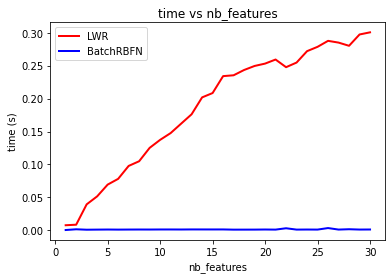
\includegraphics[width=\textwidth]{lwr_vs_rbfn_time.png}
	\captionof{figure}{Temps de calcul de LWR et BRBFN en fonction du nombre de features.}
	\label{fig:lwr_vs_rbfn_time}
\end{minipage}
\hfill
\begin{minipage}{.45\textwidth}
	\centering
	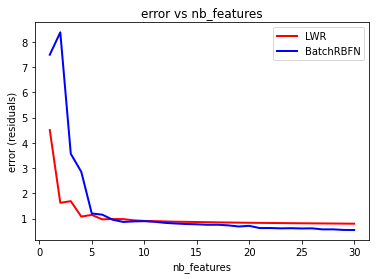
\includegraphics[width=\textwidth]{lwr_vs_rbfn_error.png}
	\captionof{figure}{Erreur de LWR et BRBFN en fonction du nombre de features.}
	\label{fig:lwr_vs_rbfn_error}
\end{minipage}
\begin{minipage}{.45\textwidth}
	\centering
	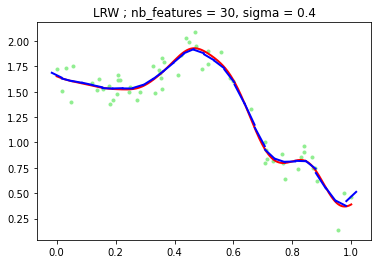
\includegraphics[width=\textwidth]{lwr_vs_rbfn_overfitting1.png}
	\captionof{figure}{Prédiction de LWR pour\\ 20 features.}
	\label{fig:lwr_vs_rbfn_overfitting1}
\end{minipage}
\hfill
\begin{minipage}{.45\textwidth}
	\centering
	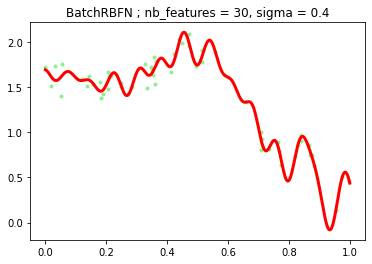
\includegraphics[width=\textwidth]{lwr_vs_rbfn_overfitting2.png}
	\captionof{figure}{Prédiction de Batch RBFN pour\\ 30 features.}
	\label{fig:lwr_vs_rbfn_overfitting2}
\end{minipage}
\end{figure}

Les figures ci-dessus permettent de souligner l'influence du nombre de features et du bruit sur LWR et Batch RBFN. Nous avons réalisé ces tests à partir d'un batch de 60 points avec plus de bruit que d'habitude ($\sigma = 0.4$).\\
Comme on peut le constater, LWR est moins sensible que RBFN face à une augmentation du bruit (Figure \ref{fig:lwr_vs_rbfn_error}). LWR est plus performant avec un nombre de features faible (entre 1 et 5), et semble mieux réagir  là où RBFN va fortement overfitter.
\`A partir de 20 features, Batch RBFN a moins de résidus que LWR puisqu'il overfit (Figures \ref{fig:lwr_vs_rbfn_overfitting1} et \ref{fig:lwr_vs_rbfn_overfitting2}).

Malgré cet avantage, le temps de calcul de LWR reste bien plus important que celui de RBFN (Figure \ref{fig:lwr_vs_rbfn_time}) qui semble négligeable en comparaison.

\newpage
\section{Neural Networks}

\begin{itemize}
		\item comment on the difference of results between the batch version, the incremental version and the incremental version with mini-batches
		\item by measuring the loss function, study the evolution of the final loss and the training time depending on the size of the minibatch, for a constant budget of iterations
		\item add a training set, a validation set and a test set, and study overfitting
\end{itemize}
\bigskip

\begin{figure}[ht]
\centering
\begin{minipage}{.33\textwidth}
	\centering
	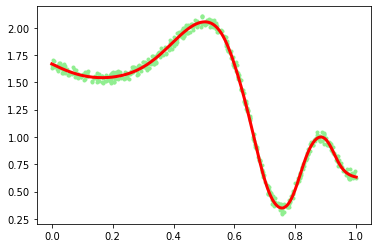
\includegraphics[width=\textwidth]{nn_batch.png}
	\captionof{figure}{Batch :\\
		- loss: 7.966e-04\\
		- time: 5.90s}
	\label{fig:nn_batch}
\end{minipage}
\hfill
\begin{minipage}{.33\textwidth}
	\centering
	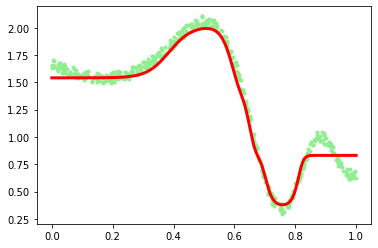
\includegraphics[width=\textwidth]{nn_incr.png}
	\captionof{figure}{Incremental :\\
		- loss: 1.154e-02\\
		- time: 29.00s}
	\label{fig:nn_incr}
\end{minipage}\hfill
\begin{minipage}{.33\textwidth}
	\centering
	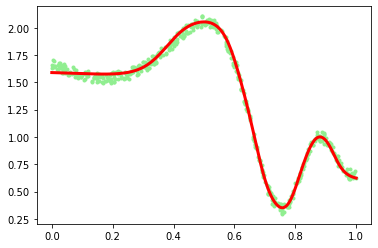
\includegraphics[width=\textwidth]{nn_incr_mb.png}
	\captionof{figure}{Mini-batches :\\
		- loss: 2.129e-03\\
		- time: 5.94s}
	\label{fig:nn_incr_mb}
\end{minipage}
\end{figure}

A partir de ces figures on remarque que la version batch est la plus précise des trois. De façon analogue aux anciens algorithmes, avec un batch complet, l’information en entrée est maximale. Le résultat est donc plus précis (Figure \ref{fig:nn_batch}).

La version incrémentale à batch constant est la moins précise (Figure \ref{fig:nn_incr}) puisqu'elle ne prend qu'une nouvelle information à la fois. Il faut donc énormement d'itérations pour qu'elle puisse apprendre les données du batch, ce qui implique un temps de calcul beaucoup trop long.

La version avec minibatch (Figure \ref{fig:nn_incr_mb}), quant à elle prend pour chaque itération un set de données un plus conséquent (50 dans notre exemple), lui permettant d'être plus rapide et plus précise.

\begin{figure}[ht]
\centering
\begin{minipage}{.45\textwidth}
	\centering
	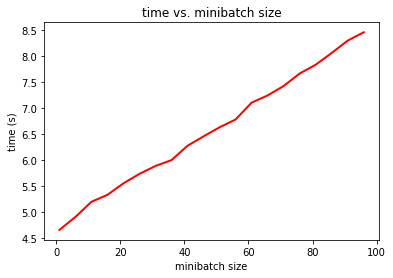
\includegraphics[width=\textwidth]{mini-batch_time.png}
	\captionof{figure}{Temps de calcul en fonction de la taille du minibatch.}
	\label{fig:mini-batch_time}
\end{minipage}
\hfill
\begin{minipage}{.45\textwidth}
	\centering
	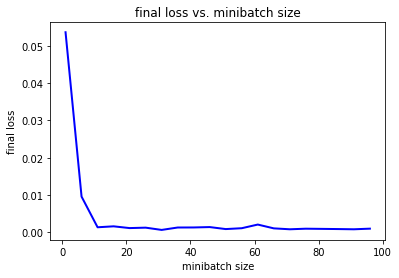
\includegraphics[width=\textwidth]{mini-batch_loss.png}
	\captionof{figure}{Erreur en fonction de la taille du minibatch.}
	\label{fig:mini-batch_loss}
\end{minipage}
\end{figure}

Si nous regardons plus en détail l'algorithme basé sur les minibatch, on peut voir que son temps de calcul dépend linéairement de la taille du minibatch. En effet, à chaque itération, plus on va rajouter des données provenant de notre minibatch à notre modèle, plus il sera long de faire le calcul (on se rapproche de la version Batch). On peut voir qu'augmenter la taille du minibatch a une grosse influence sur les loss finales.

Ce résultat est logique puisque si l'on met plus de données dans notre minibatch, notre modèle arrivera à convergence avec un nombre d'itérations fixé (5000 dans notre cas). Tandis que si l'on prend un minibatch trop petit notre modèle n’arrivera pas à convergence (après nos 5000 itérations), ce qui explique des loss finales aussi grandes dans ce cas là.

\bigskip

Nous laissons en Annexes le code de permettant la création des différents sets (training, validation, test). Nous continuons à train notre modèle tant que la loss obtenue en phase de validation ne converge pas à $10^4$ près.

\newpage
\section{Annexes}

\subsection*{La classe CustomBatch}

La manipulation du bruit (paramètre sigma) est codée en dur dans le générateur de points de la classe \lstinline{Batch}. Pour palier à ce problème nous avons récoder une version customisée de cette classe afin d'avoir plus de contrôle sur le bruit lors de la génération de points. Le $\sigma$ est maintenant un paramètre propre à la classe que l'on peut modifier lors de la création du batch. Pour nous simplifier la vie, la génération de points se fait directement dans la classe.
\bigskip

\begin{lstlisting}[language=Python]
import math
from typing import Tuple

class CustomBatch:
    def __init__(self, sigma=0.1):
        self.x_data = []
        self.y_data = []
        self.sigma = sigma
        self.c0 = np.random.random()*2
        self.c1 = -np.random.random()*4
        self.c2 = -np.random.random()*4
        self.c3 = np.random.random()*4

    def reset_batch(self) -> None:
        self.x_data = []
        self.y_data = []

    def add_non_linear_sample(self) -> Tuple[float, float]:
        x = np.random.random()
        y = self.generate_non_linear_samples(x)
        self.x_data.append(x)
        self.y_data.append(y)
        return x, y

    def generate_non_linear_samples(self, x):
        y = self.c0 - x - math.sin(self.c1 * math.pi * x ** 3) * math.cos(self.c2 * math.pi * x ** 3) * math.exp(-x ** 4)
        noise = self.sigma * np.random.random()
        y_noisy = y + noise
        return y_noisy

    def make_nonlinear_batch_data(self, size=50) -> None:
        self.reset_batch()
        for i in range(size):
            x = np.random.random()
            y = self.generate_non_linear_samples(x)
            self.x_data.append(x)
            self.y_data.append(y)
\end{lstlisting}

\subsection*{Plot helpers}

Pour simplifier l'affichage de nos analyse, nous avons ajouté les fonctions \lstinline{plot_measure(x,y,...)} qui réalise un simple plot de $\mathbf{y}$ en fonction de $\mathbf{x}$, et \lstinline{plot_mean_std(x,y,...)} qui affiche la moyenne et la variance de $\mathbf{y}$ en fonction de $\mathbf{x}$.
\bigskip

\begin{lstlisting}[language=Python]
def plot_measure(x,y,title,xlabel,ylabel,color='red',xlim=None,ylim=None,label=''):

    plt.plot(x, y, lw=2, color=color, label=label)
    plt.title(title)
    plt.xlabel(xlabel)

    if xlim: plt.xlim(xlim)
    if ylim: plt.xlim(ylim)

    plt.ylabel(ylabel)

def plot_mean_std(x,y,title,xlabel,ylabel,color='red',axis=1,xlim=None,ylim=None,label=''):

    mean = np.mean(y,axis=axis)
    std = np.std(y,axis=axis)

    plot_measure(x, mean, title, xlabel, ylabel, color, xlim, ylim, label)
    plt.fill_between(x, mean+std, mean-std, facecolor=color, alpha=.2)
\end{lstlisting}

\subsection*{Question 1}

\begin{lstlisting}[language=Python]
times = [[],[]]
cpt = 0
nb_rep = 1

for _ in range(nb_rep):
    batch = Batch()
    size = 50
    batch.make_linear_batch_data(size)
    model = LinearModel(size)

    x = np.array(batch.x_data)
    y = np.array(batch.y_data)

    start = time.process_time()
    model.train(x, y)
    times[0].append( time.process_time() - start )

    tmp = model.theta

    start = time.process_time()
    model.train_from_stats(x, y)
    times[1].append( time.process_time() - start )

    cpt += int(np.allclose(tmp,model.theta))

means = np.mean(times, axis=1)

print("LLS average time: {:.3e}s".format(means[0]))
print("LLS from scipy stats average time: {:.3e}s".format(means[1]))
print("results proximity (tolerance of 1e-08): {:.0%}".format(cpt/nb_rep))
\end{lstlisting}

\subsection*{Question 2}

\begin{lstlisting}[language=Python]
batch = Batch()
batch.make_linear_batch_data(size)
model = LinearModel(size)

coefs = [10 ** (n) for n in range(-3,4)]
lines = []

for coef in coefs:
    model.train_regularized(batch.x_data, batch.y_data, coef)
    xs = np.linspace(0.0, 1.0, 1000)
    z = model.f(xs)
    lines.append((xs, z))

plot_coef_impact(batch.x_data, batch.y_data, lines, coefs) 
\end{lstlisting}
\bigskip

\noindent Pour afficher l'impact du paramètre \lstinline{coef} sur la précision de LRR nous utilisons la fonction suivante :
\bigskip

\begin{lstlisting}[language=Python]
def plot_coef_impact(x_data, y_data, lines, coefs):
	plt.plot(x_data, y_data, 'o', markersize=3, color='lightgreen')

	norm = mpl.colors.LogNorm(vmin=min(coefs), vmax=max(coefs))
	cmap = mpl.cm.ScalarMappable(norm=norm, cmap=mpl.cm.Reds)
	cmap.set_array([])

	for i, (xs,z) in enumerate(lines):
		plt.plot(xs, z, lw=2, color=cmap.to_rgba(coefs[i]))

	cbar = plt.colorbar(cmap)
	cbar.ax.set_ylabel('coef')
	plt.title("coef impact on the accuracy of LRR")
	plt.show()
\end{lstlisting}

\subsection*{Question 3}

\begin{lstlisting}[language=Python]
times = [0,0]
nb_repet = 1000

for _ in range(nb_repet):
    batch = Batch()
    batch.make_nonlinear_batch_data(size=60)
    
    model1 = BatchRBFN1(nb_features=10)

    start = time.process_time()
    model1.train(batch.x_data, batch.y_data)
    times[0] += time.process_time() - start
    
    model2 = BatchRBFN2(nb_features=10)

    start = time.process_time()
    model2.train(batch.x_data, batch.y_data)
    times[1] += time.process_time() - start

print("First strategy average time: {:.3e}s".format(times[0] / nb_repet))
print("Second strategy average time: {:.3e}s".format(times[1] / nb_repet))
\end{lstlisting}

\subsection*{Question 4}

\begin{lstlisting}[language=Python]
features_sizes = [i for i in range(1,31)]
measures = reset_measures()

batch = Batch()

for i, nb_features in enumerate(features_sizes):
	compare_rbfns(batch, 500, nb_features, measures)

plot_comparison(measures, features_sizes, 'number of features')
\end{lstlisting}

\subsection*{Question 5}

Pour cette partie nous utilisons plusieurs fonctions facilitant la comparaison des modèles selon différents paramètres. Le dictionnaire \lstinline{measures} permet de stocker le temps et l'erreur de chaque modèle.

Au final, nous avons choisi de ne pas utiliser les graphiques représentant l'erreur en fonction du temps.

\newpage
\begin{lstlisting}[language=Python]
colors = ['red','orange','blue']
rbfns = ['RLS', 'RLS SM', 'grad descent']

def analyse_rbfn(clazz, batch, nb_features, max_iter, measures, clazz_index, func_name="train", **args):
    model = clazz(nb_features=nb_features)
    start = time.process_time()
    for i in range(max_iter):
        x, y = batch.add_non_linear_sample()
        getattr(model, func_name)(x, y, **args)

    measures["time"][clazz_index].append( time.process_time() - start )
    measures["error"][clazz_index].append( model.compute_error(batch.x_data, batch.y_data) )

def compare_rbfns(batch, max_iter, nb_features, measures):
    analyse_rbfn(RLSRBFN, batch, nb_features, max_iter, measures, 0)
    analyse_rbfn(RLSRBFN, batch, nb_features, max_iter, measures, 1, func_name="train_rls_sherman_morrison")
    analyse_rbfn(GDRBFN, batch, nb_features, max_iter, measures, 2, alpha=0.5)

def plot_comparison(measures, x, xlabel):
    for measure, data in measures.items():
        mean = np.mean(data, axis=1)
        print(f"{measure} mean: {mean}")
        for i in range(3):
            plt.plot(x, data[i], lw=2, color=colors[i], label=rbfns[i])

        plt.title(measure + ' vs. ' + xlabel)
        plt.xlabel(xlabel)
        plt.ylabel(measure)
        plt.legend()
        plt.show()

def reset_measures():
    return {
        "time":  [ [], [], [] ],
        "error": [ [], [], [] ]
    }


batch = Batch()
measures = reset_measures()

features_sizes = [i for i in range(1,31)]
for i, nb_features in enumerate(features_sizes):
    compare_rbfns(batch, 500, nb_features, measures)
plot_comparison(measures, features_sizes, 'number of features')
samples_sizes = [i for i in range(10,1001,10)]
measures = reset_measures()
for max_iter in samples_sizes:
    compare_rbfns(batch, max_iter, 10, measures)
plot_comparison(measures, samples_sizes, 'number of samples')


sigmas = [ i/10. for i in range(1, 11) ]
measures = reset_measures()
for sigma in sigmas:
    batch = CustomBatch(sigma=sigma)
    compare_rbfns(batch, max_iter, 10, measures)
plot_comparison(measures, sigmas, 'amount of noise (sigma)')
\end{lstlisting}

\subsection*{Question 7}

\noindent Evolution de l'erreur de LWR en fonction du nombre de features : 
\bigskip
\begin{lstlisting}[language=Python]
nb_features = [i for i in range(1,31)]
errors = [ [] for _ in range(len(nb_features))]

for _ in range(10):
    batch = Batch()
    batch.make_nonlinear_batch_data(60)
    for i, N in enumerate(nb_features):
        model = LWR(nb_features=N)
        model.train(batch.x_data, batch.y_data)
        errors[i].append(model.compute_error(batch.x_data, batch.y_data))

plot_mean_std(nb_features, errors, "residuals of LWR vs. the number of features", "nb_features", "error (residuals)")
\end{lstlisting}
\bigskip

\noindent Visualisation de l'impact du nombre de features sur LWR : 
\bigskip

\begin{lstlisting}[language=Python]
batch = Batch()
batch.make_nonlinear_batch_data(60)

for nb_features in [10, 20, 30, 40]:
    model = LWR(nb_features=nb_features)
    model.train(batch.x_data, batch.y_data)
    model.plot(batch.x_data, batch.y_data, f"nb_features = {nb_features}")
\end{lstlisting}
\bigskip

\noindent Comparaison de l'overfit entre LWR et Batch RBFN : 
\bigskip

\begin{lstlisting}[language=Python]
nb_features = 30
sigma = .4
batch = CustomBatch(sigma=.4)
batch.make_nonlinear_batch_data(60)

model = LWR(nb_features=30)
model.train(batch.x_data, batch.y_data)
model.plot(batch.x_data, batch.y_data, f"LRW ; nb_features = {nb_features}, sigma = {sigma}")

model = BatchRBFN1(nb_features=30)
model.train(batch.x_data, batch.y_data)
model.plot(batch.x_data, batch.y_data, f"BatchRBFN ; nb_features = {nb_features}, sigma = {sigma}", gaussians=False)
\end{lstlisting}
\bigskip

\noindent Comparaisons performance / erreur entre LWR et Batch RBFN : 
\bigskip

\begin{lstlisting}[language=Python]
features_steps = [i for i in range(1, 31)]
times = [[], []]
errors = [[], []]

for nb_features in features_steps:
    start = time.process_time()
    model = LWR(nb_features=nb_features)
    model.train(batch.x_data, batch.y_data)
    times[0].append(time.process_time() - start)
    errors[0].append(model.compute_error(batch.x_data, batch.y_data))

    start = time.process_time()
    model = BatchRBFN1(nb_features=nb_features)
    model.train(batch.x_data, batch.y_data)
    times[1].append(time.process_time() - start)
    errors[1].append(model.compute_error(batch.x_data, batch.y_data))

plt.plot(features_steps, times[0], lw=2, color='red', label="LWR")
plt.plot(features_steps, times[1], lw=2, color='blue', label="BatchRBFN")
plt.title("time vs nb_features")
plt.xlabel("nb_features")
plt.ylabel("time (s)")
plt.legend()
plt.show()

plt.plot(features_steps, errors[0], lw=2, color='red', label="LWR")
plt.plot(features_steps, errors[1], lw=2, color='blue', label="BatchRBFN")
plt.title("error vs nb_features")
plt.xlabel("nb_features")
plt.ylabel("error (residuals)")
plt.legend()
plt.show()

\end{lstlisting}

\subsection*{Question 8}

\noindent Apprentissage sur un set de training, de validation, et de test :

\begin{lstlisting}[language=Python]
set_types = [0, 0.6, 0.8, 1]

def make_minibatch_set(minibatch_size, x_data, y_data, batch_size, set_type):
    start = int(set_types[set_type-1] * batch_size)
    stop = int(set_types[set_type] * batch_size)

    xm, ym = [], []
    for i in range(minibatch_size):
        index = randrange(start, stop)
        xm.append([batch.x_data[index]])
        ym.append([batch.y_data[index]])
    return np.array(xm), np.array(ym)

batch = Batch()
batch_size = 500
batch.make_nonlinear_batch_data(batch_size)

minibatch_size = 50
model = NeuralNetwork(1, 30, 50, 50, 1, learning_rate=0.03)
start = time.process_time()

lamda = 1e-4
last_valid_loss = float("inf")

while True:
    xt, ym = make_minibatch_set(minibatch_size, batch.x_data, batch.y_data, batch_size, 1)
    yt = th.from_numpy(ym).float()
    train_output = model.f(xt)
    train_loss = func.mse_loss(train_output, yt)
    model.update(train_loss)

    xv, ym = make_minibatch_set(minibatch_size, batch.x_data, batch.y_data, batch_size, 2)
    yv = th.from_numpy(ym).float()
    valid_output = model.f(xv)
    valid_loss = func.mse_loss(valid_output, yv)

    if math.isclose(valid_loss, last_valid_loss, rel_tol=lamda):
        break

    model.update(valid_loss)
    last_valid_loss = valid_loss

xtest, ym = make_minibatch_set(minibatch_size, batch.x_data, batch.y_data, batch_size, 3)
ytest = th.from_numpy(ym).float()
loss = func.mse_loss(valid_output, ytest)

print("NN Incr minibatch Reg final loss: {:.3e}".format(loss.item()))
model.plot(xv, ytest)
\end{lstlisting}

\subsection*{Résultat intriguant}

\begin{figure}[h]
\centering
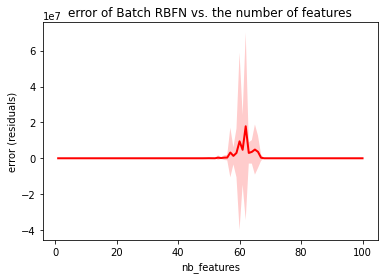
\includegraphics[width=.45\textwidth]{batch_rbfn_error_vs_n_features100.png}
\captionof{figure}{Evolution du temps de calcul de RLS\\ pour un nombre de features allant de 1 à 100.}
\label{fig:batch_rbfn_error_vs_nfeat100}
\end{figure}

Lors de l'analyse de l'impact du nombre de features sur la précision de RLS, nous remarquons un pic d'erreurs absurde, de l'ordre de $10^7$, aux alentours de 60 features (Figure \ref{fig:batch_rbfn_error_vs_nfeat100}).

\end{document}